% This is samplepaper.tex, a sample chapter demonstrating the
% LLNCS macro package for Springer Computer Science proceedings;
% Version 2.21 of 2022/01/12
%
\documentclass[runningheads]{llncs}
%
\usepackage[T1]{fontenc}
\usepackage{graphicx}
\usepackage{hyperref}
\usepackage{color}
\usepackage{charter}
\usepackage{amsmath}
\usepackage{semantic}
\usepackage{caption}
\usepackage{subcaption}

\newcommand{\ctyp}[2]{C^{#1}#2}
\newcommand{\imult}{\oplus}
\newcommand{\iunit}{\mathsf{e}}

\renewcommand\UrlFont{\color{blue}\rmfamily}
\urlstyle{rm}

\newcommand{\T}{Tomas}
\newcommand{\J}{Joel}
\newcommand{\says}[2][gg]{\vspace{0.5em}\noindent\hangindent=0.5cm{\textsc{#1}}: #2}
\newcommand{\appears}[3][gg]{\vspace{0.5em}\noindent\hangindent=0.5cm{\textsc{#1}} (\emph{#2}): #3}

\begin{document}

\title{On the Limits of Making Programming Easy}
\titlerunning{On the Limits of Making Programming Easy}

\author{Tomas Petricek\inst{1} \and
Joel Jakubovic\inst{2}}
\authorrunning{T. Petricek, J. Jakubovic}

\institute{Charles University, Prague, Czechia\\
\email{tomas@tomasp.net} \and
University of Kent, Canterbury, UK\\
\email{joel.jakubovic@cantab.net} }

\maketitle

\begin{abstract}
A lot of programming research shares the same basic motivation: how can we make programming easier? Alas, this problem is difficult to tackle directly. Programming is a tangle of conceptual models, programming languages, user interfaces and more and we cannot advance all of these at the same time. Moreover, we have no good metric for measuring whether programming is easy. As a result, we usualy give up on the original motivation and pursue narrow tractable research for which there is a rigorous methodology.

\qquad In this paper, we investigate the limits of making programming easy. We use a dialectic method to circumscribe the design space within which easier programming systems may exist. In doing so, we not only bring together ideas on open-source software, self-sustainable systems, visual programming languages, but also the analysis of limits by Fred Brooks in his classic ``No Silver Bullet'' essay. We sketch a possible path towards easier programming of the future, but more importantly, we argue for the importance of proto-theories as a method for tackling the original motivating basic research question.

\keywords{Programming systems \and complexity \and technical dimensions.}
\end{abstract}

\section{Introduction}
A cold winter morning, 1st December 2023, outside the Cambridge Computer Laboratory; two computer scientists arrive in the area known as The Street in front of the lecture theaters; they aim to attend the MycroftFest symposium: Tomas Petricek---a former PhD student of Alan---and Joel Jakubovic, Tomas’ PhD student. The elder and younger researchers discuss threads of programming study as different from each other as The Street and the Cambridge Computer Laboratory are from Trinity Street and Peterhouse.

Let's eavesdrop.

~

~

~

~

\section{Programming systems}

\says[\T]{I hope you are ready for your PhD defense next week, Joel! The examiners will surely ask you to give a brief summary of your work, so you'll need a good answer for that. Have you figured out how to summarize what your PhD work is about?}

\says[\J]{I always like to introduce it as making programming ``suck less!'' I suppose I will need something that sounds more formal than that. Of course, I mean it in a very focused and specific way that is small enough to fit into a PhD.}

\says[\T]{My PhD was about making programming easier too. I worked on client-server web programming before~\cite{petricek-2007-fswebtools} and found it tricky to keep track of the right context on the two sites. Some code requires resources that are only available on the server (e.g. a database), while some requires resources only available in the web browser (e.g. the user's location).}

\says[\J]{So what did you do to make client-server web programming easier?}

\says[\T]{I tried to fix this by designing a context-aware programming language that would track the context requirements, or \emph{coeffects}, in the type system~\cite{petricek-2013-coeffects}. With coeffects, the type would tell you not just what your functions take and return, but also that some part of your code can run only on some of the sites.}

\says[\J]{And did that make programming easier?}

\says[\T]{Well, I ended up looking mostly at other use cases (dataflow, liveness) and only ever built a prototype implementation of a  language with coeffect support.\footnote{The prototype can be found, in the form of an interactive essay, at \url{https://tomasp.net}.} But if someone implemented a proper language based on the theory, then I believe it would make programming client-server web applications easier...}


\begin{figure}[t]
\vspace{-0.5em}
\centering
\begin{equation*}
\boxed{\begin{array}{c}
\\[-0.5em]
\inference[(\emph{var})\;]
  {x : \tau \in \Gamma}
  {\ctyp{\iunit}{\Gamma} \vdash x : \tau }
%
\quad\quad
%
\inference[(\emph{app})\;]
  {\ctyp{r}{\Gamma} \vdash e_1 : \ctyp{t}{\tau_1} \rightarrow \tau_2 &
   \ctyp{s}{\Gamma} \vdash e_2 : \tau_1 }
  {\ctyp{r \vee (s \imult t)}{\Gamma} \vdash e_1~e_2 : \tau_2}
\\[1.2em]
\inference[(\emph{sub})\;]
  {\ctyp{s}{\Gamma} \vdash e : \tau }
  {\ctyp{r}{\Gamma} \vdash e : \tau }
\;(s\leq r)
%
\quad\quad\quad\quad
%
\inference[(\emph{abs})\;]
  {\ctyp{r \wedge s}{(\Gamma, x:\tau_1)} \vdash e : \tau_2}
  {\ctyp{r}{\Gamma} \vdash \lambda x.e : \ctyp{s}{\tau_1} \rightarrow \tau_2 }
\\[-0.5em]~
\end{array}}
\end{equation*}

\vspace{0.5em}
(a) Type and coeffect system for tracking context requirements \cite{petricek-2013-coeffects}.
\vspace{1.5em}

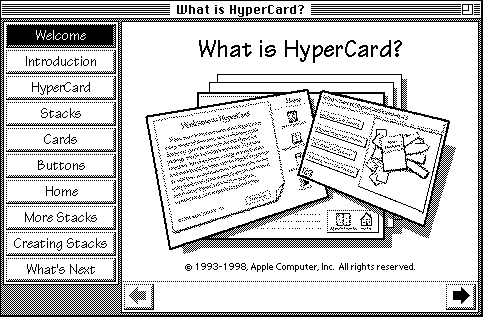
\includegraphics[scale=0.7]{figures/hyper.png}

\vspace{0.5em}
(b) A screenshot of Hypercard, an early hypertext system that allowed \\
users to easily create their own interactive ``decks''.
\vspace{0.5em}

\caption{The contrast between programming languages and programming systems. We know how to study \emph{languages} (a), but not how to study \emph{systems} (b). }
\label{fig:langsys}
\vspace{-0.5em}
\end{figure}

\says[\J]{Oh dear... so your work was only concerned with improving programming \emph{languages}.}

\says[\T]{Of course. Programming languages are the medium through which you program. But you make it sound like you have something else in mind.}

\says[\J]{We both say that we are interested in making \emph{programming} easier. Programming is about much more than programming languages and their formal properties. We should be thinking about programming \emph{systems} more generally, not just about languages (see Figure~\ref{fig:langsys}).}

\says[\T]{What is the difference? What is a programming system?}

\says[\J]{A programming \emph{language} is an abstract formal entity. A programming \emph{system} is a running, interactive and stateful collection of software. A system may implement a language (or multiple languages). It includes a runtime and a compiler or an interpreter, but it also consists of graphical interfaces used to edit code, debug code and so on.}

\says[\T]{I'm still not convinced. Of course you need to write your code and invoke the compiler in some way. That's why you also have a terminal and Emacs to do programming.}

\says[\J]{You are thinking about the problem through the lens of the \emph{languages} paradigm. The point is that the \emph{systems} paradigm gives you a different perspective, different problems and different research methods. Gabriel wrote about this in his ``Structure of a Programming Language Revolution'' \cite{rpg-2012-revolution}, where he points out that there was a paradigm shift through the 1990s from thinking about systems to thinking about languages. This encouraged more formal academic work on programming, but Gabriel also explains how some good ideas about programming became unthinkable because of this shift.}

\says[\T]{You can say that a programming language plus all the extra things it needs is a programming system, but what other good ideas about programming does this view enable?}

\says[\J]{First, the different view lets us consider ways to make programming easier which are hard to think about as languages. For example, visual programming, block-based editing \cite{resnick-2009-scratch} or systems like Flash \cite{ankerson-2018-dot} and Hypercard. These are programming systems we should learn from. Second, the view lets us talk about interactivity and self-sustainable systems that can be modified from within themselves \cite{hirschfeld-2008-s3,hirschfeld-2010-s3}. It would be useful to understand highly malleable programming systems like Lisp and Smalltalk, because they can in principle be used to make their \emph{own} programming easier.}

\says[\T]{But Lisp and Smalltalk are languages ... ah, I see what you're going to say. Smalltalk-the-system \emph{contains} Smalltalk-the-language, but a lot of other important things like its interface! And similarly for systems built on Lisp...}

\says[\T]{Those are very good points. I'm starting to believe that this programming systems view is actually useful. But let's return to it later, because I wanted to return to one more point you made...}

\section{Essential complexity}

\says[\T]{You said that the goal of your work was to make programming easier. I can see how thinking about programming systems rather than programming languages is a better way to approach the problem. Yet, I worry that this may not be as much help as you hope. Didn't Fred Brooks came up with an argument showing that you cannot make programming an order of magnitude easier?}

\says[\J]{Interesting, why did he think that?}

\says[\T]{Brooks \cite{brooks-1987-silver} analysed the different kinds of complexity involved in building software. The \emph{essential complexity} is inherent in the real-world. It comes from the fact that our software has to encode the many (perhaps ad-hoc) rules of the human world. The \emph{accidental complexity} comes from imperfection in our tools and languages.}

\says[\T]{Now, Brooks argues that we can reduce the accidental complexity through better tools, but the essential complexity will remain. He then points out that we will not be able to get an order of magnitude improvement in overall complexity of software unless the accidental complexity in software today is more than 10x that of the essential complexity.}

\says[\J]{This may have been a valid point in the 1980s, but it assumes a very Waterfall view of software development. You only have to tackle the essential complexity all at once if you are designing a system from scratch. Not all programming is about that.}

\says[\T]{Programming methodologies have certainly evolved since Brooks' time. Today, you might use Agile methods rather than Waterfall, but I think the basic idea holds. You still have to construct the entire system with all its essential complexity.}

\says[\J]{Well, I know you like to relate software development to architecture \cite{petricek-2021-architecture}, so perhaps that can help me explain what I'm thinking.}

\says[\T]{Even more than in software, in architecture, you have to manage all the complexity and build the whole house! You can rely on modernist analysis or the traditional "unselfconscious" way of building that the early Christopher Alexander favoured \cite{alexander-1964-notes}, but you need to solve all the design problems the house involves.}

\begin{figure}[t]
\centering
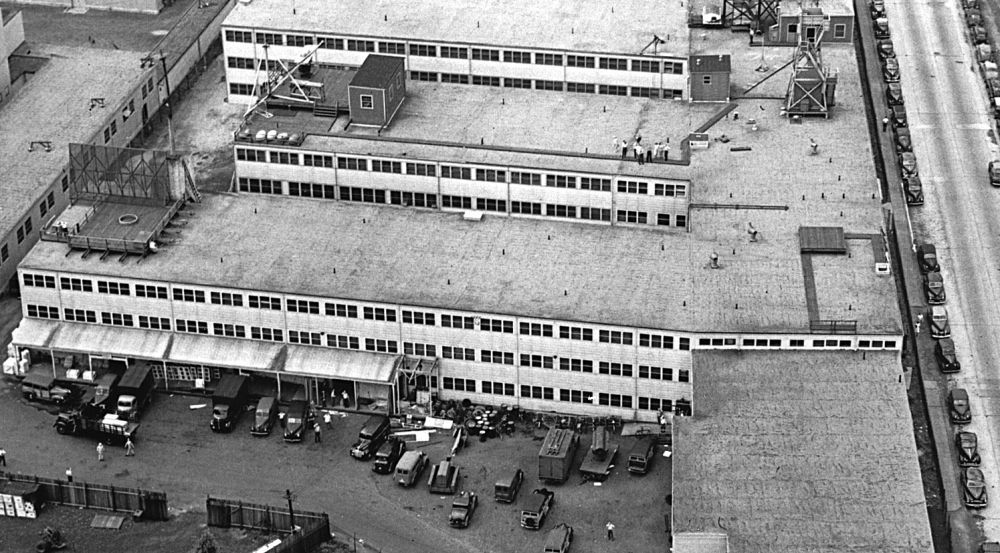
\includegraphics[scale=0.33]{figures/mit20.jpg}
\caption{MIT Building 20 was a temporary timber building, erected for radar research during the World War II. It continued to exist for over 50 years and was highly popular for its infinite
adaptability \cite{brand-1994-buildings} (photo: MIT Museum).}
% https://www.ll.mit.edu/about/history/mit-radiation-laboratory
\label{fig:mit20}
\end{figure}

\says[\J]{I think you can look at the problem very differently though. As argued by Stewart Brand \cite{brand-1994-buildings}, buildings also evolve. Old power stations become galleries, a garage becomes a co-working space, while a formal city plaza suddenly gains new use as an ice-skating rink \cite{cohen-1974-context}. Even when the spaces are not designed for their future use, they often end up fitting it remarkably well.}

\says[\T]{You are probably right. Buildings seem like the most static things, yet they evolve. Software, being structured information, ought to be much more malleable than the rigid materials of buildings; accordingly, it evolves much faster. But how can this solve the problem of software complexity?}

\says[\J]{Like buildings, I think we often build software by gradual adaptation. We may not always think about it that way, but we should embrace this view. Very often, you have software that does \emph{almost} what you want, but not quite.}

\says[\T]{I guess systems that you can buy and configure, like SAP that was slowly rising to prominence when Brooks was writing his paper \cite{leimbach-2008-sap}, would be an interesting example of that.}

\says[\J]{This is not quite what I had in mind, but fair enough! The point is, I think we can sidestep Brooks' ``doom prophecy'' by focusing on how software is built by making small changes to existing software. To make software development easy, we should make it easy to make \emph{changes!} }

\says[\T]{Wait a second! Isn't building software in this way, through a sequence of small adaptations, something that the free software community already thought of in the 1980s? Having access to code and freedom to change it was the whole point of free software. The free software manifesto says you should have ``The freedom to study how the program works, and \emph{change it so it does your computing as you wish}.''\cite{fsf-2001-whatis}}

\says[\J]{In theory, yes, but does access to source code really give you the freedom to change a program as you wish for any moderately complex open-source software today?}

\says[\T]{I think you are right. The complexity of most software that we are dealing with today means that, even as a hacker myself, I cannot hope to understand and modify software with a reasonable amount of effort, even if I do have the source code.}

\says[\J]{In fact, this probably worked in the 1980s when the GNU utilities were a manageable size and all the users were hackers who could modify and compile the code!}

\says[\T]{Isn't this inevitable? The kind of sofware we need today is just more complex, because computers get used for more complex problems. We are facing Brooks' essential complexity again. To make a small change to a large piece of software, you may not need to understand all of it, but you need to understand a significant part of it and even that is prohibitive. }

\section{Programming that scales}

\says[\J]{Isn't it inevitable that static source code simply doesn't scale for understanding complex dynamic systems? The change we want to make is to the dynamic behaviour, but we have to trace the causality backwards and figure out which change to the \emph{initial} state will produce it. At today's scales, this is like being a surgeon forced to operate on the DNA and then regrow the entire patient. Who would expect this to work?}

\says[\T]{Isn't the whole point of programming to tackle this kind of complexity through abstractions? Going back to my own PhD, a key idea in it was that you can hide multiple fairly complex specific instances of context-dependence behind a simple unified mathematical structure.}

\says[\J]{Many computer scientists like to see programming as a formal mathematical activity, but this is just a metaphor and it has its limits. De Millo, Lipton and Perlis
pointed this out in 1979 \cite{demillo-1979-proofs}! They believed that formal verification of software is bound to fail, because the complexity of the formal entities \emph{computer scientists} work with is different than the complexity of the formal entities \emph{mathematicians} work with. A mathematical proof is probably correct because mathematicians excitedly go over it on a whiteboard with their colleagues, but no such social process accompanies formal proofs of software.\footnote{For a detailed and a refined account of the debate that followed the publication of the paper, as well as the historical context, see the book written by MacKenzie~\cite{mackenzie-2001-proof}.}}

\says[\T]{If seeing programs as formal mathematical entities is not the right perspective, then what is the alternative?}

\says[\J]{In the early 2000s, the Software Engineering Institute at Carnegie Mellon University asked this very question as part of their project on Ultra-large-scale systems \cite{feiler-2006-ulss} They said that we need to shift how we think about problems we face and that new perspectives will by inspired by work looking at disciplines such as microeconomics, biology, city planning, and anthropology.}

\says[\T]{I do like the city planning metaphor for thinking about software. If you look how people understand a city, as documented in the classic book ``The image of the city'' \cite{lynch-1960-image}, I think much of that applies to source code. If you want to get from one place to another in a city, you do not need to understand the whole city. There are paths through the city that take you there like, for example, the metro line. Is this what you are thinking about?}

\says[\J]{You can surely alleviate some of the scaling problems with source code by organising it better, but it is still wrong to have to search through the source code and look for names that sound like the right thing, in order to find the relevant code for the change we want to achieve.}

\says[\T]{What do you imagine, then?}

\says[\J]{Well, a programming system should model the chain of cause to effect in programs that you create. Then, when you want to make a change to something that you can see, or to something that produces visible outputs or effects on the screen, it can point you back to the code that you need to change. Bret Victor demonstrated what this could look like \cite{bret-victor}, but I'm unaware of any follow-up work to realise his vision---which raises the question of how he himself got his demo to work, something that does occasionally keep me up at night.}

\says[\T]{I think I can imagine the technical characteristics such a system would need to work: it would need to record information about its execution and make it acessible. Basman \cite{basman-2022-materialized} refers to this idea as ``materialized execution'' and traces it to the 1980s Boxer project \cite{disessa-1986-boxer}. A similar idea was also used recently to automatically link data visualizations by analysing code used to produce them \cite{perera-2022-galois}.}

\says[\J]{This is useful technical background, but we should also look to interesting \emph{real} programming systems---not just demos---for inspiration about interfaces that would make such program editing accessible.}

\says[\T]{Perhaps the various live and exploratory programming systems \cite{rein-2018-live} may be relevant here?}

\says[\J]{Yes, those tools give you rapid feedback. Perhaps a surprisingly good example here is Excel, which also, to some extent, keeps track of the chain of cause to effect in that you can view the source of the formula and see which other cells were used to compute the result. You do have to backtrace the causal chain manually by looking up the cells one by one. But it is the best example I can think of.}

\says[\T]{In fact, Excel has pretty good backtracing support now! But regardless of whether you trace manually or with the system's help, this only works with the relatively simple formula language. If you want to achieve some more complicated behaviour, you have to do that with VBA macros and give up this traceability. }

\begin{figure}[t]
\centering
\begin{subfigure}{0.48\textwidth}
   \noindent
   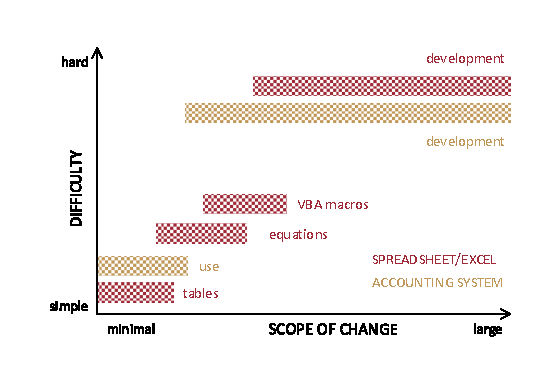
\includegraphics[scale=0.65]{figures/sub1.pdf}
   \caption{Excel offers multiple but disconnected substrates (data entry, formulas, macros).}
   \label{fig:sub1}
\end{subfigure}
\hfill
\begin{subfigure}{0.48\textwidth}
   \noindent
   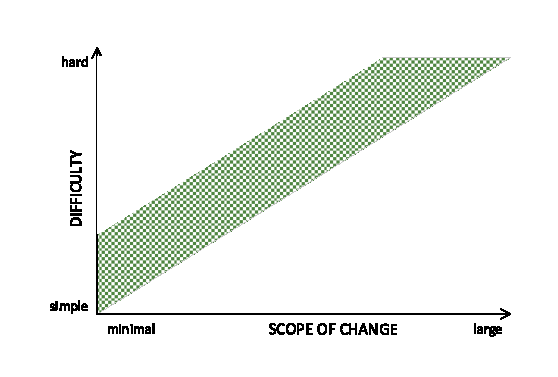
\includegraphics[scale=0.65]{figures/sub2.pdf}
   \caption{An ideal system would have one adaptable substrate that makes minimal changes simple, but allows harder larger chages.}
   \label{fig:sub2}
\end{subfigure}
\caption{Scope of change vs. difficulty of use of multiple programming substrates.}
\label{fig:substrates}
\end{figure}

\section{Programming substrates and notations}

\says[\J]{True, so let's stop to think about notations for a bit. We can understand them better by charting the scope of change that can be achieved through a particular notation against the difficulty of using the notation. Figure~\ref{fig:sub1} shows this for a hypothetical accounting system and a spreadsheet system.}

\says[\T]{I see. For an accounting system, you have the graphical interface that provides a notation for using the system and a notation (say, Java or C++) with which the system is implemented. For a spreadsheet, you have tables where you enter your data, formulas, VBA macros and then the notation used to implement Excel itself.}

\says[\J]{Right. This is already better than regular software, because there are appropriate notations for changes at multiple difficulty levels, but it is not perfect...}

\says[\T]{There is perhaps a nice characterization of the ideal notational continuum that we are looking for in the work of Pierre Depaz \cite[p.123]{depaz-2023-aesthetics} on aesthetics of code. He says that \emph{``simplicity is found in source code when the syntax and the ontologies used are an exact fit to the problem: simple code is code that is neither too precise, nor too generic, displaying an understanding of and a focus on the problem domain, rather than the applied tools.''}}

\says[\J]{I think this really boils down to two things. First, to be able to use the right tools for different jobs, you need to be free from a restriction to just one notation. Second, you should also be free from a restriction to plain text; non-textual notations should be on the menu, because those are sometimes the most appropriate fit for a problem.}

\says[\T]{Hmm, but wouldn't such a ``notational pluralism'' be impractical? In Excel, you may use multiple disjoint notations such as tables, formulas and macros---yet this also means that there is no gradual progression between them. If you learn how to use formulas, it does not help you at all with learning how to write macros (or even become a developer working on Excel at Microsoft...).}

\says[\J]{Yes, the right approach seems to be to have an adaptable substrate. Something that has a basic form, but can be adapted in various ways to suit particular domain-specific problems. See the illustration in Figure~\ref{fig:sub2} where the same (adaptable) substrate can be used for both small and simple changes, but also large and (inevitably) difficult changes.}

\says[\T]{But how would this work? You would need a substrate where an end-user can make a small change and gradually progress. The starting point then has to be something they are already familiar with. To take a spreadsheet as an example, do you think the substrate could somehow ``grow'' from filling numbers in a table to modifying some simple aspects of the system that users may care about, like making the interface color scheme colour blind friendly or making the wording of menu items clearer?}

\says[\J]{Something like this could work in spreadsheets. I can think of some parts of Excel-the-application that transfer well to a portion of a spreadsheet. One could press a button to ``reflect'' the key/value pairs in the preferences menu into two columns of cells. When edited, these cells would update Excel's internal preferences that you normally edit in a dialog box. At a stretch, perhaps other parts of such a dialog could also be reflected---say, the list of options in a drop-down box. And then you could, for example, have your preferences computed with formulas!}

\says[\T]{Hmm, are you getting at some general principle with this idea?}

\says[\J]{The notation for development should resemble the notation for use!}

\begin{figure}[t]
\centering
\begin{minipage}[t]{0.4\textwidth}\vspace{0pt}
  
\includegraphics[scale=0.27]{figures/piet.png}
\end{minipage}
\begin{minipage}[t]{0.5\textwidth}\vspace{0pt}
  \caption{``Hello world'' program in the esoteric programming language Piet. The program instructions are encoded as colours and are executed as a pointer moves over the individual colour regions of the bitmap.}
  \label{fig:piet}
\end{minipage}
\end{figure}

\says[\T]{Well, this is a heavy constraint on the notations we can use for development! What would justify such an idea?}

\says[\J]{I admit, it's about as restrictive as one could get! The motivation is that the user is already familiar with the ``notation for use'' in the software---so to the extent that ``development'' can be massaged to use the same notation, they are able to adapt the software by re-using the same skills. They no longer have to invest in learning a completely different notation (like a programming language) before they can do that.}

\says[\T]{So, to take this idea to its limits, you're saying that MS Paint should be written in the Piet esolang that we can see in Figure~\ref{fig:piet}?!}

\says[\J]{Fair enough. I wouldn't go so far; *given that* the use-notation in Paint is what it is, there aren't many changes to Paint that fit sensibly within it. That being said---the program's tool icons could be ``reflected'' in its canvas and re-drawn that way, but that's the only straw I can think to grasp! The principle will break down with absurd examples if you commit to it fully, but that doesn't mean we shouldn't explore its domain of validity. It is still promising, but you need to think about what really is the essence of the substrate through which most people interact with computers today. It is not pixels...}

\says[\T]{Do you mean buttons, tabs, tables, lists, forms and such?}

\says[\J]{I believe there is a more fundamental substrate behind all of those. You can model a lot of user interface widgets as rigid bodies that exist in some space, connected with rods and springs and perhaps forces such as attraction and repulsion between particular entities.}

\says[\T]{How do you imagine this would provide a programming substrate?}

\says[\J]{I do not have a perfect answer to this question, but you can think of the basic substrate as a sort of ``user interface physics'' within which specific visual notations for particular problems could be defined.\footnote{Constraint-based systems for specifying user interfaces, such as Cassowary \cite{borning-1997-constraints}, can be seen as related to this idea, although they focus more on rendering the layout for the end-user than on developing a foundational underlying substrate. Additionally, individual constraints are too low-level for a human-friendly UI substrate, although they could well be what such a substrate ``compiles'' to in order to run. This was the subject of much research in the 1990s \cite{myers-1992-uilangs}.} Such a substrate could even be the result of taking a 2D physics engine, stripping it of concepts like mass and rotations, and optimising it for this simpler domain. If we had that, then I think we would make a step towards the ideal substrate for programming. And the substrate would need to live within an actual running materialized system, rather than a static blueprint like a program in source code today.}

\section{Research methodologies}

\says[\T]{You certainly have some very interesting ideas about the future of programming here, but let me ask an annoying practical question. How do you turn this into a realistic research project? Is there something you can analyse formally or measure about a prototype? To make this into a research agenda, there needs to be some scientific methodology behind it!}

\says[\J]{Tomas, remind me, didn't you run into a problem in your thesis with the intersection of provable and interesting things?}

\says[\T]{Well, you remember correctly. There was a point in my PhD when I realized that all the things I could prove about my programming language were not that interesting, and all the things that I found interesting about programming were not particularly formalizable or provable. I guess I was getting increasingly interested in what people sometimes call ``programming experience'' research.\footnote{The topic is the subject of the Programming Experience workshop\\ (https://programming-experience.org) that has been running since 2016.} The experience also made me think much more about research methodology and led me to interest in history and philosophy of science.}

\says[\J]{Does that shed any light on why programming language researchers are so focused on formalization and proofs?}

\says[\T]{Well, for one thing, there is a bias for theory over experiment in all branches of science. Ian Hacking \cite{hacking-1983-representing} pointed this out in the case of physics, as did Hossenfelder \cite{2018-hossenfelder-lost}, and the same applies to computer science. However, finding a suitable methodology for programming experience research is an open problem that does not have a definite answer. It may need a range of qualitative and quantitative methods, including formalisms and empirical evaluation, but also system descriptions, user studies and perhaps even interactive artifacts \cite{edwards-2019-eval}.}

\says[\J]{I do not understand how you are supposed to make general and unifying claims if you do not first start by looking at the concrete and specific!}

\says[\T]{Indeed, and there are two examples of this that come to mind. For most of its history, particle physics consisted of two sub-cultures that Peter Galison refers to as the ``image'' and ``logic'' traditions \cite{galison-1997-image}. While the latter focused on statistical analysis of observations, the former attempted to capture ``golden events'' that show the decay of a single particle. These concrete traces went on to be hugely influential in shaping the theory of particle physics. And in the case of city planning, Jane Jacobs made a similar argument \cite{jacobs-1961-death} in favor of looking at specific cases, which she calls ``unaverage clues''. An example is a chain of bookshops that always remain open until late, except for one branch in Brooklyn. The clue tells you something significant about that part of the city.}

\says[\J]{OK, but on reflection, we need something in between. In order to do any formalisation or a user study, you need conceptual clarity on what you're studying and what you're trying to find out. I don't think we have any such clarity on many interesting aspects of programming systems.}

\says[\T]{But what kind of knowledge structure can give you such conceptual clarity, without being as detailed as a formal model?}

\begin{figure}[t]
\vspace{-0.5em}
\centering
\begin{subfigure}{0.49\textwidth}
  \centering
   \noindent
   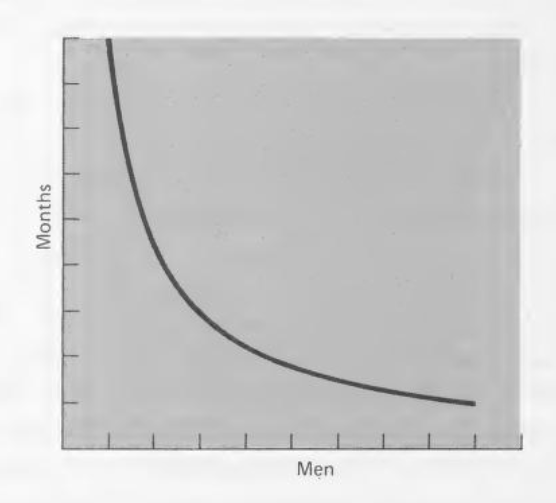
\includegraphics[scale=0.3]{figures/mm1.png}
   \caption{Time versus number of workers:\\Perfectly partionable task}
   \label{fig:xx}
\end{subfigure}
\hfill
\begin{subfigure}{0.49\textwidth}
  \centering
   \noindent
   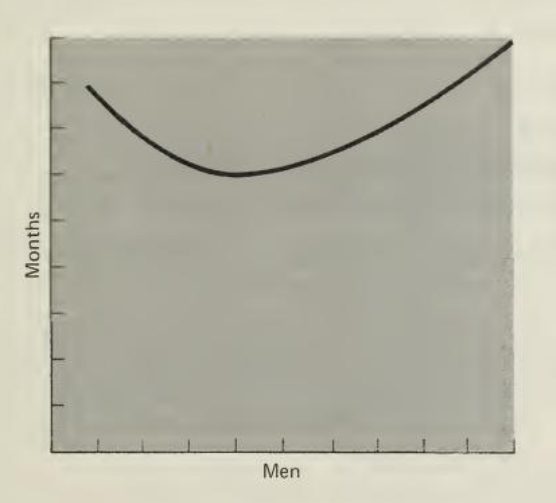
\includegraphics[scale=0.3]{figures/mm2.png}
   \caption{Time vs. number of workers:\\Task with complex inter-relationships}
   \label{fig:syy}
\end{subfigure}
\caption{Two illustrations by Brooks showing how communication overhead means that adding workforce to a delayed project makes things worse (from~\cite{brooks-1975-manmonth})}
\label{fig:mm}
\vspace{-0.5em}
\end{figure}

\says[\J]{You made a reference to Fred Brooks earlier. I think his other essay ``The Mythical Man-Month'' \cite{brooks-1975-manmonth} is a good example. In the essay, Brooks explains why adding more workforce to a delayed project only makes the delay worse. The argument is based on analysing the amount of communication that needs to happen (Figure~\ref{fig:mm}). For a perfectly partitionable programming task, adding people helps. But if the work requires communication, the overhead of the communication grows exponentially as people are added, eventually overtaking the gain you get from the linear growth of people who can do the programming. Brooks illustrates this with charts and equations. He does not have formal proofs or specific numbers, but the model provides a good theory that provides conceptual clarity.}

\says[\T]{Interesting, this kind of reasoning seems to be quite common in software engineering. I can think of another example from a book about the history of anti-ballistic missile systems \cite{slayton-2013-arguments}. One of the arguments for why such systems cannot be reliably built was based on comparing the rate of change in the environment and the rate of change of the system. The idea was that the US cannot build a reliable defence system, because changing the software takes more work than changing some of the characteristics of the Soviet missiles. Ergo, their defences won't be able to keep pace with Soviet innovations in offensive capability. Again, this is a somewhat mathematical argument that provides conceptual clarity.}

\says[\J]{Right. I think we can refer to such models that provide conceptual clarity \emph{proto-theories}. I would say that we need more thinking like this! They can be later refined to more formal models, but not prematurely. I would also add that mathematical formulations like those above are not the only kinds of proto-theories we should be creating.}

\says[\T]{So what would be a useful proto-theory about programming systems?}

\section{Technical dimensions of programming systems}

\says[\J]{Well, a good place to start would be the published framework of ``technical dimensions''
\cite{jakubovic-2023-techdims} which break down programming systems into narrower properties of which they can have more or less.}

\says[\T]{Dimensions? That rings a bell...}

\says[\J]{You're thinking of the Cognitive Dimensions of Notations \cite{green-1990-cogdims} which was the main inspiration. However, the Technical Dimensions are concerned with the programming system as a whole, not just its notation.}

\says[\T]{I can see how you capture various properties of notations. They can be more or less
  dense, more or less consistent, more or less easy to modify etc. But what kind of properties
  can you capture as dimensions about programming systems in general?}

\says[\J]{The list is quite long and I do not think it is complete, but it includes some of the
  characteristics of programming systems that we have talked about already. For example,
  \emph{modes of interaction} captures whether you do everything in a single environment or
  whether ``using'' is distinct from ``programming''; \emph{notational structure} captures whether
  there is just a single adaptable notation or a range of different ones; \emph{self-sustainability}
  captures the degree to which the system can be modified from within itself and so on.}

\says[\T]{Just to get back to our original question, how does such a framework contribute to making programming easier?}

\says[\J]{Remember Figure~\ref{fig:langsys}, which illustrated that we know how to study programming languages, but not how to study programming systems? Well, many people came up with interesting programming systems that make programming easier in some way. But because we lacked a good way for talking about them, the ideas were never clearly described and nobody was able to adopt them and develop them further.}

\says[\T]{I guess what you are saying is that technical dimensions of programming systems gives us a set of common points of reference that allow for apples-to-apples comparison of widely different programming systems? But is this meant to supersede the existing programming language research methods?}

\says[\J]{Not at all. Since many programming systems contain a programming language, all existing programming language research is applicable to their syntax, semantics, types, paradigms, and so on. The technical dimensions simply establish the analogues of those concepts for the other parts of those systems.}

\says[\T]{Didn't you link the change from thinking about programming languages to thinking about programming systems to the idea of Kuhnian paradigm shift before?}

\says[\J]{Yes, it would be a corrective to the shift that Gabriel observed in the opposite direction\ \cite{rpg-2012-revolution}; not by \emph{fighting} PL research, but by simply making space to do the more general thing. To truly establish a new paradigm, the return to thinking about systems would put more emphasis on research methods that can talk about them in their full complexity. It would not \emph{invalidate} programming language theory, but it could make it more of a speciality instead of the default. However, we are quite far from what Kuhn called ``normal science''. It is still early days for programming systems research!}

\says[\T]{What do you think still needs to be done? I have to say that, compared to established programming language research methods, the work on technical dimensions seems quite informal!}

\says[\J]{Right. The full realisation of the aims of the framework is a long-term research program. What we have already is the seed to start it off. We have a set of dimensions that come with qualitative descriptions. Future work, as set out towards the end of my dissertation \cite{jakubovic-2024-phd}, involves making these descriptions more precise and possibly even quantifiable.}

\says[\T]{Quantifiable? Does this risk the problem we mentioned about focusing on what is formalizable rather than on what is interesting?}

\says[\J]{That spectre is always hanging over it, yes. But the solution is to refine the framework slowly and carefully, with input and critique from the research community. This is why the dimensions were published in their qualitative state; better to grit our teeth and endure the informality, than to prematurely formalise before we know what we're doing! Just the fact that we're breaking down programming systems into a common vocabulary of properties to focus on, helps to analyse programming systems and compare them with each other. It also means we can map the design space of possible systems and spot combinations of properties that haven't been tried yet.}

\says[\T]{It is funny to hear us discussing the theoretical framework of programming systems, after we complained about the scientific bias in favour of theoretical work! You have just outlined the future work for interested ``theoreticians'', but the future work for ``experimentalists'' should be at least as important. I guess the experimental work should be filling the database of how different systems fit into the framework.}

\says[\J]{That is certainly one task for the experimentalists. But they can also explore the design space to find new designs. To get back to our original motivation of making programming easier, my thesis explores programming systems that have three properties: \emph{notational freedom}, which would give you the kind of adaptable substrate we talked about,
\emph{explicit structure}, which is a pre-condition for building such a substrate, and
\emph{self-sustainability}, which would make it possible to evolve the system from
within itself, enabling a virtuous cycle of self-improvement.}

\section{Conclusions}

\appears[Alan]{arrives in his festive Christmas jumper}{\textsc{Ho Ho Ho!} It is nice to see you! What have you two been chatting about here?}

\says[\T]{Well, Joel was practicing the elevator pitch for his PhD thesis, but we got a bit distracted. We ended up talking about whether it is possible for programming to be easier, whether there are any fundamental limits to that, and also what kind of research methodology can get us there!}

\says[Alan]{And what did you conclude?}

\says[\J]{On a more general level, we agreed that we need more thinking about interactive, stateful programming systems and their characteristics. Programming can only become easier if we start thinking about how programming systems are used. In other words, think more about \emph{programming systems} than about \emph{programming languages}. Today, this is tricky, because we lack the right vocabulary for talking about programming systems, but the technical dimensions are a useful \emph{proto-theory} that serves as the starting point!}

\says[Alan]{And on the more specific level?}

\says[\J]{Well, we do not have a concrete system yet, but we believe it will have a number of general properties. It needs to be built around a programming substrate that can grow with the user. It should make it easy to make small changes to the system, but also allow making more complex and difficult changes. We also need to think about programming as gradual adaptation, to overcome Brooks' ``doom prophecy'' of essential complexity. But I remain optimistic.}

\says[\T]{My tongue-in-cheek suggestion is that your
\emph{Concepts in Programming Languages} module, which I very much enjoyed back in the day, should become
\emph{Concepts in Programming Systems}! We need a new generation of programming systems researchers who will adopt this new way of thinking about programming and come up with great new theories and experimental systems!}

\says[Alan]{So, what do you think the next generation of Computer Lab programming systems PhD students should be doing?}

\says[\J]{I would love to see more research that looks at how programming languages are embedded in broader stateful interactive systems. This is something where we are lacking both theory and new interesting design ideas. I also think programming researchers should look at things that we do not really see as programming languages. What is it that makes systems like Excel, but also Flash, Hypercard or game engines work well as programming tools? We also need to be more fearless in looking at problems that are interesting, but informal. If we are to study informal properties that are not simply true or false, we will also need more focus on finding consensus among researchers working on programming tools, such as agreeing on the right proto-theories on which to further advance our work.\footnote{A recent seminar also focused on the problem of developing new ``theories of programming'' \cite{latoza-2023-theories}. However, we believe that a theory needs to start as an informal proto-theory and that \emph{premature} scientific framing in terms of hypotheses may inhibit progress.}}

\begin{credits}
\subsubsection{\ackname}
The events portrayed in this essay are entirely fictional. Any resemblance to actual persons, living or dead, is purely coincidental. But we are grateful to the non-fictional people who participated in a lively discussion at Mycroftfest and helped to shape this essay.
~
This study was supported by X (grant number Y).
\end{credits}

\bibliographystyle{splncs04}
\bibliography{paper}

\end{document}
